\documentclass[tikz]{standalone}
% Default preamble
\usepackage{pgfplots}
\pgfplotsset{compat=newest}
\usepgfplotslibrary{groupplots}
\usepgfplotslibrary{polar}
\usepgfplotslibrary{smithchart}
\usepgfplotslibrary{statistics}
\usepgfplotslibrary{dateplot}
% Custom preamble from global variable:
\usepgfplotslibrary{fillbetween}
\begin{document}
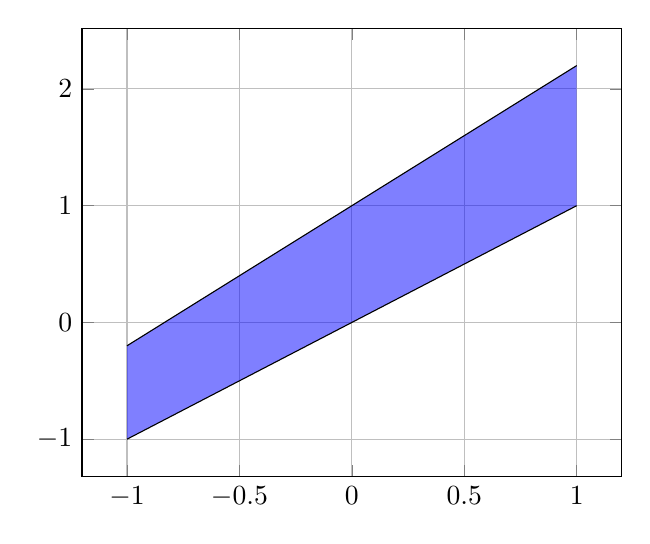
\begin{tikzpicture}
\begin{axis}[xmajorgrids, ymajorgrids]
    \addplot[name path=f, no marks]
        coordinates {
            (-1.0,-1.0)
            (-0.96,-0.96)
            (-0.92,-0.92)
            (-0.88,-0.88)
            (-0.84,-0.84)
            (-0.8,-0.8)
            (-0.76,-0.76)
            (-0.72,-0.72)
            (-0.68,-0.68)
            (-0.64,-0.64)
            (-0.6,-0.6)
            (-0.56,-0.56)
            (-0.52,-0.52)
            (-0.48,-0.48)
            (-0.44,-0.44)
            (-0.4,-0.4)
            (-0.36,-0.36)
            (-0.32,-0.32)
            (-0.28,-0.28)
            (-0.24,-0.24)
            (-0.2,-0.2)
            (-0.16,-0.16)
            (-0.12,-0.12)
            (-0.08,-0.08)
            (-0.04,-0.04)
            (0.0,0.0)
            (0.04,0.04)
            (0.08,0.08)
            (0.12,0.12)
            (0.16,0.16)
            (0.2,0.2)
            (0.24,0.24)
            (0.28,0.28)
            (0.32,0.32)
            (0.36,0.36)
            (0.4,0.4)
            (0.44,0.44)
            (0.48,0.48)
            (0.52,0.52)
            (0.56,0.56)
            (0.6,0.6)
            (0.64,0.64)
            (0.68,0.68)
            (0.72,0.72)
            (0.76,0.76)
            (0.8,0.8)
            (0.84,0.84)
            (0.88,0.88)
            (0.92,0.92)
            (0.96,0.96)
            (1.0,1.0)
        }
        ;
    \addplot[name path=g, no marks]
        coordinates {
            (-1.0,-0.1999999999999999)
            (-0.96,-0.15200000000000008)
            (-0.92,-0.10400000000000002)
            (-0.88,-0.05599999999999999)
            (-0.84,-0.007999999999999948)
            (-0.8,0.04000000000000009)
            (-0.76,0.08800000000000002)
            (-0.72,0.13600000000000007)
            (-0.68,0.184)
            (-0.64,0.23200000000000004)
            (-0.6,0.2800000000000001)
            (-0.56,0.328)
            (-0.52,0.37600000000000006)
            (-0.48,0.424)
            (-0.44,0.47200000000000003)
            (-0.4,0.52)
            (-0.36,0.5680000000000001)
            (-0.32,0.616)
            (-0.28,0.664)
            (-0.24,0.712)
            (-0.2,0.76)
            (-0.16,0.808)
            (-0.12,0.856)
            (-0.08,0.904)
            (-0.04,0.952)
            (0.0,1.0)
            (0.04,1.048)
            (0.08,1.096)
            (0.12,1.144)
            (0.16,1.192)
            (0.2,1.24)
            (0.24,1.288)
            (0.28,1.336)
            (0.32,1.384)
            (0.36,1.432)
            (0.4,1.48)
            (0.44,1.528)
            (0.48,1.576)
            (0.52,1.6239999999999999)
            (0.56,1.672)
            (0.6,1.72)
            (0.64,1.768)
            (0.68,1.816)
            (0.72,1.8639999999999999)
            (0.76,1.912)
            (0.8,1.96)
            (0.84,2.008)
            (0.88,2.056)
            (0.92,2.104)
            (0.96,2.152)
            (1.0,2.1999999999999997)
        }
        ;
    \addplot[thick, color={blue}, fill={blue}, opacity={0.5}]
        fill between [of=f and g]
        ;
\end{axis}
\end{tikzpicture}
\end{document}
